\chapter{General State of the Art}


\section{Context}

To replace materials that are very practical but very problematic for our environment, convince people of the usefulness of the replacement. on the one hand, by making functional objects. But also by opening the door to new imaginations that broaden the scope of what's possible. that's why, in the same way as classical research, design helps to shape this problem. 
\begin{marginfigure}[-5cm] % Adjust the vertical placement
    \centering
    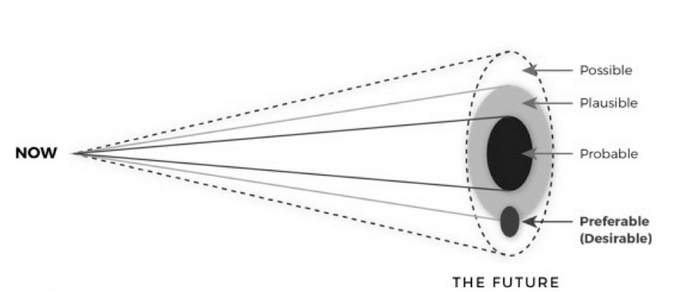
\includegraphics[width=\linewidth]{images/futures_cone.png}
    \caption{futures cone representation}
    \label{fig:futures code}
\end{marginfigure}
Science in this field relatively new. The starting point differs depending on how define biomaterials and how make, or rather grow them. 
More globally, biomaterials are at the crossroads of many fields of scientific and even artistic research. From agriculture to design, from synthetic biology to fashion, from DIY fermented drink to biohacking in the kintchen\cite{CiteTheOdin}.
This is in line with new interdisciplinary courses integrating biodesign, such as MIT's "How To Grow (Almost) Anything" course\cite{CiteMITHTGAA}. 

As matter of fact, the starting point might be the first crops domestication. At this time the goal was only to produce food, and the process were optimized by selective breeding. By taking the plants with the biggest fruit or the best resistance to environment, from generation to generation plants were "optimized" for the population.
Besides, the use of wood are very use in numerous sectors\cite{ramage2017wood} push by international directive of less CO2 emmission and waste. 
  
However, today, biomaterials or biobased materials in this study are more in line with the aim of replace existing materials like plastics.
This biomaterials production projects are aimed to create in the futures of cone plausible or possible futures. 
Moreover the development of this new materials go hand in hand with the evolution of new machines for biomaterials. Bioreactors are controlled environment systems. There is no notable differences in hardware part from bioreactors in the litterature. The general form is a isolated space from outside environmental conditions, 
combine with a controler responsible of sensors and actuator (i.e :fogger, fan, thermal resistance...). The controler is also responsible to send data when monitoring is wanted. All powered by energy from different sources. 

Multiple reviews\cite{cottet2020biobased}\cite{vinod2020renewable}\cite{hairon2022bio} about biobased materials support for the fact that today's synthetic materials, especially those derived from oil, are a problem for human and ecosystem health.
These studies reveals the strong interess of these materials in term of sustainability and low cost production, and "by reducing wastages, landfills
and toxic emissions leading to greener and cleaner environment". They also show end proprieties these materials are distinguished by their biodegradability and compostability. Which also makes them interesting for their end-of-life properties. 
However, there are concers about a lack of large scale industrialisation and a lack standadise methodology \cite{andrew2022sustainable}. This leads to a lack of confidence in mechanical properties, as the absence of standardization, give rise to the limited exploitation of technical data on characteristics such as tensile strength, compression, fatigue, impact resistance and flammability, makes assessment more difficult.   
Into the bargain, most of these materials are and highly anisotropic.

\paragraph[short]{Industry} 
Ecovative and MycoWorks lead in mycelium-based biomaterials. Ecovative creates eco-friendly alternatives to plastics for packaging and construction, while MycoWorks focuses on sustainable mycelium leather, targeting fashion and luxury markets.
\paragraph[short]{In Design} 
Suzanne Lee, through Biofabricate, pioneers biofabrication in design, using biological processes to grow sustainable materials like microbial leather, pushing the boundaries of traditional manufacturing and eco-conscious design.


\section{Biomaterial}
\subsection{S.C.O.B.Y Lether} 

\paragraph[short]{Definition } 
S.C.O.B.Y, aim to Symbiotic Culture Of Bacteria and Yeast, during this symbiotic culture a lot of biochimical element are tranformed or exchanged by bacteria and yeast.
Among this biochimical elements, there is bacterial cellulose. Bacterial cellulose (BC) is a biopolymer that grows on the surface of the culture medium. 

More precisely, 2 metabolic processes are at play, in a kind of “double” fermentation. 
on the one hand, alkolic fermentation by leaven. In other words, the glucoses (C_6H_{12}O_6) will be converted into ehtanol (CH_3CH_2OH). 
on the other hand, “acetic fermentation” by bacteria. In other words, the ethanol(CH_3CH_2OH) will be converted into acetic acid.

C_6H_{12}O_6 + 2 \, \text{ADP} + 2 \, P_i \rightarrow 2 \, \text{ATP} + 2 \, H_2O + 2 \, \textcolor{red}{CH_3CH_2OH} + 2 \, CO_2

\textcolor{red}{CH_3CH_2OH} + O_2 \rightarrow CH_3COOH + H_2O

\begin{figure}[h]
    \centering
    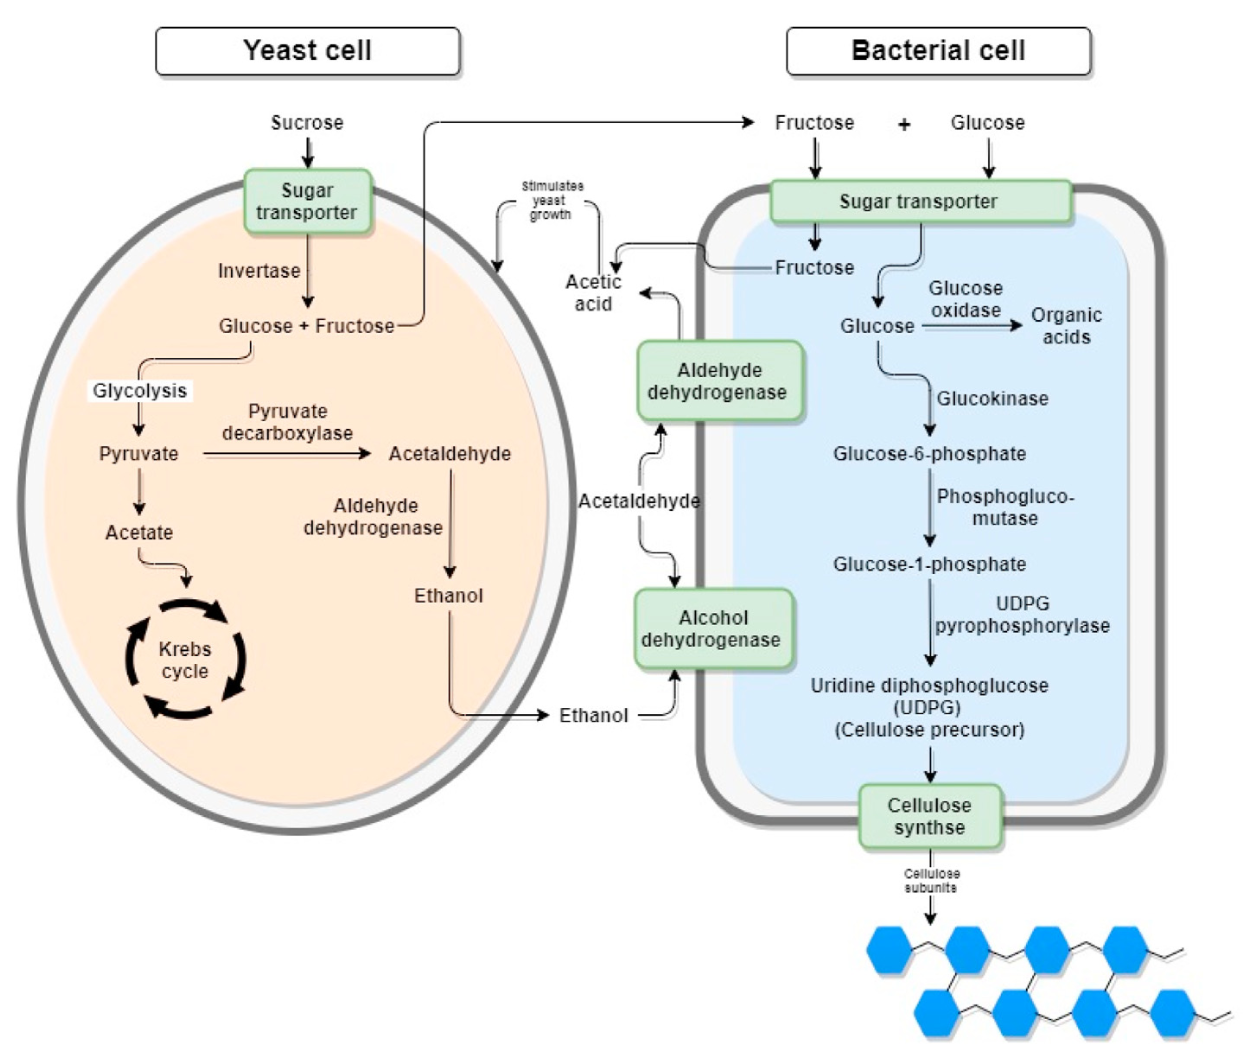
\includegraphics{images/schema_metabolique.png}
    \caption{Metabolism of substrates by the symbiotic culture of bacteria and yeast from\cite{laavanya2021current}}
    \label{fig:metabolic}
\end{figure}

in addition to the metabolic processes that allow these microorganisms to survive and reproduce, bacteria will also synthesize this so-called bacterial cellulose.




\paragraph[short]{Use}

\subsection{Mycelium}


\subsection{Other Biomaterial}




















\section{Bioreactor \& Controlled Environment }

\subsection{Controlled Environment} 



















\subsection{Bioreactor}
\subsection{Bioreactor S.C.O.B.Y}
\subsection{Bioreactor Mycelium}



\section{Discution and limitation}